\documentclass[12pt]{article}

\usepackage[a4paper,margin=2cm]{geometry}

\usepackage{amsmath}
\usepackage{amssymb}
\usepackage{mathtools}

\usepackage{listings}

\usepackage{booktabs} % For tables
\usepackage[table,xcdraw]{xcolor} % For tables

\usepackage{enumerate}
\usepackage{enumitem}

\usepackage{nameref}

\usepackage{xcolor}

\definecolor{codegreen}{rgb}{0,0.6,0}
\definecolor{codegray}{rgb}{0.5,0.5,0.5}
\definecolor{codepurple}{rgb}{0.58,0,0.82}
\definecolor{backcolour}{rgb}{0.95,0.95,0.92}

\lstdefinestyle{mystyle}{
    backgroundcolor=\color{backcolour},
    commentstyle=\color{codegreen},
    keywordstyle=\color{magenta},
    numberstyle=\tiny\color{codegray},
    stringstyle=\color{codepurple},
    basicstyle=\ttfamily\footnotesize,
    breakatwhitespace=false,
    breaklines=true,
    captionpos=b,
    keepspaces=true,
    numbers=left,
    numbersep=5pt,
    showspaces=false,
    showstringspaces=false,
    showtabs=false,
    tabsize=2
}

\lstset{style=mystyle}

\DeclarePairedDelimiter\abs{\lvert}{\rvert}
\DeclarePairedDelimiter\Abs{\lVert}{\rVert}

\usepackage{fancyhdr}

\pagestyle{fancy}
\lhead{\today}
\chead{Exercise 01\\Algorithmic Foundations of Data Science}
\rhead{Tanhim Islam\\Simon Michau\\Til Mohr}

\setlength{\headheight}{50pt}

\begin{document}

\section*{Exercise 1}
We can define the \textit{edit distance} $d_{\text{edit}}(w,w'): \Sigma^2 \rightarrow \mathbb{R}$ as follows. (Let $w=w_1 \dots w_n$ and $w'=w'_1 \dots w'_m$)

\begin{equation*}
	d_{\text{edit}}(w,w') \mapsto
	\begin{cases}
		\abs{w} & \text{if } \abs{w'}=0 \\
		\abs{w'} & \text{if } \abs{w}=0 \\
		d_{\text{edit}}(w_2 \dots w_n, w'_2 \dots w'_m) & \text{if } w_1 = w'_1 \\
		1 + \min
			\begin {cases}
				d_{\text{edit}}(w_2 \dots w_n, w') \\
				d_{\text{edit}}(w, w'_2 \dots w'_m) \\
				d_{\text{edit}}(w_2 \dots w_n, w'_2 \dots w'_m)
			\end{cases}
			& \text{otherwise}
	\end{cases}
\end{equation*}

As this definition of $d_{\text{edit}}$ works by removing at most the first character of each word, we can proof by induction the length of $x,y,z \in \Sigma$, that $d_{\text{edit}}$ is a metric on $\Sigma$:
\begin{itemize}
	\item	Let $\abs{x}=\abs{y}=\abs{z}=0$. Therefore, also $x=y=z$. \\
			Then $0 \leq d_{\text{edit}} = 0$. Thus, Nonnegativity is given. \\
			Since $x=y$, also $d_{\text{edit}}(x,y) = d_{\text{edit}}(y,x)$. Thus, Symmetry is given. \\
			Since $x=y=z$, the Triangle Inequality $d_{\text{edit}}(x,z) \leq d_{\text{edit}}(x,y) + (d_{\text{edit}})(y,z) \Leftrightarrow 0 \leq 0 + 0$ is given.
	\item 	Let $x=x_1 \dots x_n$, $y=y_1 \dots y_m$, and $z=z_1 \dots z_o$, $n,m,o \geq 1$. For $x'=x_2 \dots x_n$, $y'=y_2 \dots y_m$, and $z'=z_2 \dots z_o$ Nonnegativity, Symmetry, and the Triangle Inequality of $d_{\text{edit}}$ is given.
	\item	Since $n,m \geq 1$, the second rule of Nonnegativity, namely $d_{\text{edit}}(x,y) \Leftrightarrow x=y$ does not apply here. \\
			Since all $d_{\text{edit}}(x',y'), d_{\text{edit}}(x',y), d_{\text{edit}}(x,y')$ are non-negative, by definition of $d_{\text{edit}}$, $d_{\text{edit}}(x,y)$ must be non-negative as well. Therefore, the Nonnegativity of $d_{\text{edit}}$ is proven.
	\item	If $x_1 = y_1$, then $d_{\text{edit}}(x,y) = d_{\text{edit}}(x',y') = d_{\text{edit}}(y',x') = d_{\text{edit}}(y,x)$ \\
			If $x_1 \neq y_1$. Since there is a shortest path to convert $x$ into $y$, we can denote the order of operations as $(op_1, \dots, op_p)$. The shortest path to convert $y$ into $x$ is also of the same length and can be denoted as $(anti(op_p), \dots, anti(op_1))$, where $anti$ denotes the opposite to an operation and is defined as follows:
			\begin{align*}
				anti(ins_i^a(w_1 \dots w_{i-1} w_i w_{i+1} w_n)) & \coloneqq del_i(w_1 \dots w_{i-1} a w_{i+1} w_n) \\
				anti(del_i(w_1 \dots w_{i-1} w_i w_{i+1} w_n)) & \coloneqq ins_{i}^{w_i}(w_1 \dots w_{i-1} w_{i+1} w_n) \\
				anti(repl_i^a(w_1 \dots w_{i-1} w_i w_{i+1} w_n)) & \coloneqq repl_i^{w_i}(w_1 \dots w_{i-1} a w_{i+1} w_n)
			\end{align*}
			Thus, Symmetry is proven.
	\item	We can denote the path to convert $x$ into $y$ and the path to convert $y$ into $z$ by the order of operations $O_1 \coloneqq (op_1, \dots, op_p), O_2 \coloneqq (op'_1, \dots, op_p')$. Since $p,p' \geq 0$, since $d_{\text{edit}}$ is nonnegative, the shortest path of converting $x$ to $z$ must not be larger than $p+p'$, since $(op_1, \dots, op_p, op'_1, \dots, op_p')$ is also a valid order of operations for that purpose. Thus, the Triangle Inequality is proven.
\end{itemize}

Since $d_{\text{edit}}$ is nonnegative, symmetric, and fulfills the triangle inequality, $d_{\text{edit}}$ is a metric.

\pagebreak
\section*{Exercise 2}
Result (see \nameref{appendix} for code):
\bigskip

Classification: k=2 Manhattan Distance \\
Test (1, -2, 0): Prediction 1 \\
Test (4, -0.5, 2): Prediction -1 \\
Test (1, 1.5, -2.5): Prediction 0 \\
Test (-2, -1, -2): Prediction 0 \\
Test (-4, -1, -1): Prediction 0
\bigskip

Classification: k=3 Manhattan Distance \\
Test (1, -2, 0): Prediction 1 \\
Test (4, -0.5, 2): Prediction -1 \\
Test (1, 1.5, -2.5): Prediction 1 \\
Test (-2, -1, -2): Prediction -1 \\
Test (-4, -1, -1): Prediction 1
\bigskip

Classification: k=2 Euclidean Distance \\
Test (1, -2, 0): Prediction 1 \\
Test (4, -0.5, 2): Prediction -1 \\
Test (1, 1.5, -2.5): Prediction 1 \\
Test (-2, -1, -2): Prediction 0 \\
Test (-4, -1, -1): Prediction 0
\bigskip

Classification: k=3 Euclidean Distance \\
Test (1, -2, 0): Prediction 1 \\
Test (4, -0.5, 2): Prediction -1 \\
Test (1, 1.5, -2.5): Prediction 1 \\
Test (-2, -1, -2): Prediction 1 \\
Test (-4, -1, -1): Prediction -1
\bigskip

\subsection*{Further Reasoning}
\subsubsection*{(a),(b)}
\begin{table}[h!]
\begin{tabular}{lllllll}
\hline
Coordinate           & Label & (1,-2,0)                    & (4,-0.5,2)                  & (1,1.5,-2.5)                & (-2,-1,-2)                  & (-4,-1,-1)                     \\ \hline
(-4,-2.1,-1)         & -1    & 6.1                         & 12.6                        & 10.1                        & \cellcolor[HTML]{FFCC67}4.1                         & \cellcolor[HTML]{FFFE65}1.1    \\
(-3.6,-1.4,0.2)      & 1     & 5.3999                      & 10.3                        & 10.2                        & 4.2 & \cellcolor[HTML]{FFFE65}1.9999 \\
(1,-0.2,-0.3)        & 1     & \cellcolor[HTML]{FFFE65}2.1 & 5.6                         & \cellcolor[HTML]{FFFE65}3.9 & 5.5                         & 6.5                            \\
(0.3,-0.5,-0.5)      & 1     & \cellcolor[HTML]{FFCC67}2.7 & 6.2                         & 4.7                         & 4.3                         & 5.3                            \\
( -2, -3.5, -1)      & -1    & 5.5                         & 12.0                        & 9.5                         & \cellcolor[HTML]{FFFE65}3.5 & 4.5                            \\
(-4.2, -4, 0.2)      & 1     & 7.4                         & 13.5                        & 13.3999                     & 7.4                         & \cellcolor[HTML]{FFCC67}4.4    \\
(-1.3, -0.1, -3)     & 1     & 7.1999                      & 10.7                        & 4.4                         & \cellcolor[HTML]{FFFE65}2.6 & 5.6                            \\
(-0.7, 0.9, -0.7)    & 1     & 5.3                         & 8.8                         & \cellcolor[HTML]{FFCC67}4.1 & 4.5                         & 5.4999                         \\
( 1, 2, 1.4)         & 1     & 5.4                         & 6.1                         & 4.4                         & 9.4                         & 10.4                           \\
( 2.6, -1.5, 0.2)    & 1     & \cellcolor[HTML]{FFFE65}2.3 & 4.2                         & 7.3                         & 7.3                         & 8.2999                         \\
( 2, 4.3, -0.7)      & -1    & 8.0                         & 9.5                         & 5.6                         & 10.6                        & 11.6                           \\
( 0.6, 0.4, 0.2)     & -1    & 3.0                         & 6.1                         & 4.2                         & 6.2                         & 7.2                            \\
( 2.9, -1.7, 3.6)    & -1    & 5.8                         & \cellcolor[HTML]{FFCC67}3.9 & 11.2                        & 11.2                        & 12.2                           \\
( 3.6, 0.4, -2.5)    & -1    & 7.5                         & 5.8                         & \cellcolor[HTML]{FFFE65}3.7 & 7.5                         & 10.5                           \\
( 1.2, 4, 1.2)       & -1    & 7.4                         & 8.1                         & 6.4                         & 11.3999                     & 12.3999                        \\
( -1, 0.5, 0.5)      & -1    & 5.0                         & 7.5                         & 6.0                         & 5.0                         & 6.0                            \\
( 3, 2.7, 2.3)       & -1    & 9.0                         & 4.5                         & 8.0                         & 13.0                        & 14.0                           \\
( 4, -3, 2.2)        & -1    & 6.2                         & \cellcolor[HTML]{FFFE65}2.7 & 12.2                        & 12.2                        & 13.2                           \\
( 0.1, 0.1, 3.5)     & -1    & 6.5                         & 6.0                         & 8.3                         & 8.7                         & 9.7                            \\
( 2.8, 1.2, 2.4)     & -1    & 7.4                         & \cellcolor[HTML]{FFFE65}3.3 & 7.0                         & 11.4                        & 12.4                           \\ \hline
Classification (k=2) &       & 1                           & -1                          & 0                           & 0                           & 0                              \\
Classification (k=3) &       & 1                           & -1                          & 1                           & -1                           & 1                             \\ \hline
\end{tabular}
\caption{Manhattan distance table for the 5 query points. Classifications for k=2 (a) and k=3 (b) are stated below.}
\end{table}
\clearpage

\subsubsection*{(c),(d)}
\begin{table}[h!]
\begin{tabular}{lllllll}
\hline
Coordinate           & Label & (1,-2,0)                      & (4,-0.5,2)                    & (1,1.5,-2.5)                  & (-2,-1,-2)                    & (-4,-1,-1)                    \\ \hline
( -4, -2.1, -1)      & -1    & 5.1                           & 8.692                         & 6.341                         & \cellcolor[HTML]{FFFE65}2.491 & \cellcolor[HTML]{FFFE65}1.1   \\
(-3.6, -1.4, 0.2)    & 1     & 4.643                         & 7.862                         & 6.071                         & 2.749                         & \cellcolor[HTML]{FFFE65}1.326 \\
( 1, -0.2, -0.3)     & 1     & \cellcolor[HTML]{FFCC67}1.825 & 3.792                         & \cellcolor[HTML]{FFFE65}2.780 & 3.539                         & 5.111                         \\
( 0.3, -0.5, -0.5)   & 1     & \cellcolor[HTML]{FFFE65}1.729 & 4.465                         & 2.913                         & 2.791                         & 4.357                         \\
( -2, -3.5, -1)      & -1    & 3.5                           & 7.348                         & 6.020                         & 2.692                         & \cellcolor[HTML]{FFCC67}3.201 \\
(-4.2, -4, 0.2)      & 1     & 5.575                         & 9.095                         & 8.036                         & 4.322                         & 3.237                         \\
(-1.3, -0.1, -3)     & 1     & 4.231                         & 7.297                         & 2.846                         & \cellcolor[HTML]{FFFE65}1.516 & 3.478                         \\
(-0.7, 0.9, -0.7)    & 1     & 3.434                         & 5.598                         & \cellcolor[HTML]{FFFE65}2.547 & \cellcolor[HTML]{FFCC67}2.643 & 3.819                         \\
( 1, 2, 1.4)         & 1     & 4.238                         & 3.950                         & 3.931                         & 5.436                         & 6.305                         \\
( 2.6, -1.5, 0.2)    & 1     & \cellcolor[HTML]{FFFE65}1.688 & \cellcolor[HTML]{FFCC67}2.489 & 4.341                         & 5.123                         & 6.726                         \\
( 2, 4.3, -0.7)      & -1    & 6.417                         & 5.859                         & 3.475                         & 6.766                         & 8.011                         \\
( 0.6, 0.4, 0.2)     & -1    & 2.441                         & 3.950                         & 2.942                         & 3.682                         & 4.955                         \\
( 2.9, -1.7, 3.6)    & -1    & 4.082                         & \cellcolor[HTML]{FFFE65}2.282 & 7.145                         & 7.473                         & 8.322                         \\
( 3.6, 0.4, -2.5)    & -1    & 4.332                         & 4.606                         & \cellcolor[HTML]{FFCC67}2.823 & 5.793                         & 7.872                         \\
( 1.2, 4, 1.2)       & -1    & 6.122                         & 5.360                         & 4.469                         & 6.743                         & 7.541                         \\
( -1, 0.5, 0.5)      & -1    & 3.240                         & 5.315                         & 3.741                         & 3.082                         & 3.674                         \\
( 3, 2.7, 2.3)       & -1    & 5.602                         & 3.366                         & 5.336                         & 7.561                         & 8.577                         \\
( 4, -3, 2.2)        & -1    & 3.852                         & 2.507                         & 7.165                         & 7.592                         & 8.845                         \\
( 0.1, 0.1, 3.5)     & -1    & 4.180                         & 4.221                         & 6.226                         & 5.989                         & 6.186                         \\
( 2.8, 1.2, 2.4)     & -1    & 4.386                         & \cellcolor[HTML]{FFFE65}2.118 & 5.228                         & 6.873                         & 7.914                         \\ \hline
Classification (k=2) &       & 1                             & -1                            & 1                             & 0                             & 0                             \\
Classification (k=3) &       & 1                             & -1                            & 1                             & 1                             & -1                           \\ \hline
\end{tabular}
\caption{Euclidian distance table for the 5 query points. Classifications for k=2 (c) and k=3 (d) are stated below.}
\end{table}
\clearpage

\pagebreak
\section*{Exercise 3}
\begin{enumerate}[label=(\alph*)]
	\item	$X_1 \land X_2 \land X_3$ is obviously in $1$-CNF, thus also in $2$-CNF. There exists no satisfiability equivalent formula in $2$-DNF. For this, there would have to be at least two disjunctions of conjunctions of at most 2 literals. Thus, such a formula would be true even if one literal would be false.
	\item	$X_1 \lor X_2 \lor X_3$ is obviously in $1$-DNF, thus also in $2$-DNF. There exists no satisfiability equivalent formula in $2$-CNF. Since such a formula can only have 2 literals in each disjunction, there is no possibility of validating, that the third literal might be true. Therefore, such a formula is not true, when just one literal is true, the others false.
	\item	$k-DNF$:\\
			We make use of Theorem 1.3 (a). \\
			We can map the binary tree $t$ of height $k$ to a boolean function $f: \{0,1\}^n \rightarrow \{0,1\}$ in $k-DNF$ by following algorithm: \\
			For each path $p$ in $t$, that leads to a \verb|TRUE| classification, we can create the conjunction $c_p \coloneqq \bigwedge_{l_i \in p} l_i$, where $l_i$ is the literal of the variable $x_i$ on the path. Since $t$ is of height $k$, $p$ at most contains $k$ literals, thus $c_p$ at most contains $k$ literals. We can now define $f$ in $k-DNF$ as follows:
			\[f \coloneqq \bigvee_{p \in t} c_p = \bigvee_{p \in t} \bigwedge_{l_i \in p} l_i\]\\
			$k-CNF$:\\
			We use the above algorithm for $k-DNF$ to create a boolean function $f': \{0,1\}^n \rightarrow \{0,1\}$ in $k-DNF$, however, for this, we do only use the paths $p$ in $t$, that lead to a \verb|FALSE| classification. Therefore, $f'$ is then \verb|TRUE|, iff the decision tree $t$ classifies \verb|FALSE|.\\
			By negating $f'$, we can get our desired function $f$ in $k-CNF$:
			\[f \coloneqq \neg f' = \neg \bigvee_{p \in t} \bigwedge_{l_i \in p} l_i = \bigwedge_{p \in t} \bigvee_{l_i \in p} \neg l_i\]
\end{enumerate}


\section*{Exercise 4}
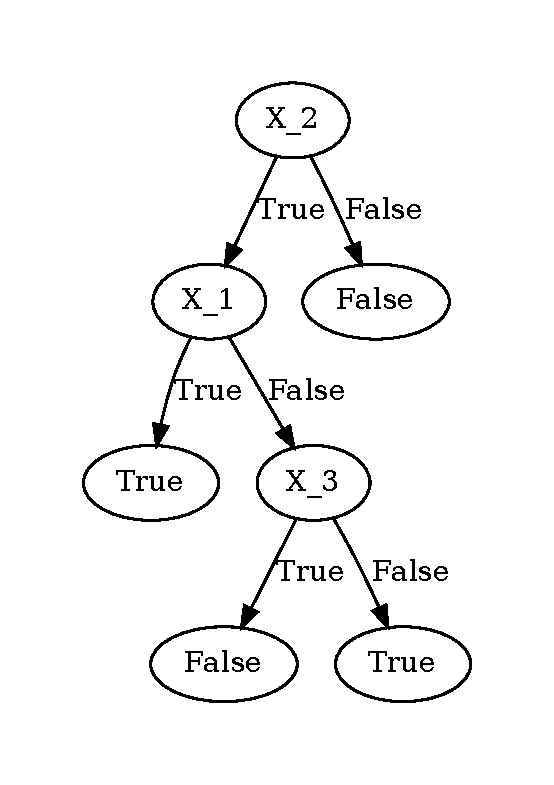
\includegraphics{code/Decision-Tree.gv.pdf} \\
Reasoning (see \nameref{appendix} for code):
\bigskip

Feature Set: $[X_1, X_2, X_3]$ \\
Gains for each feature $[(X_2, 0.5487949406953987), (X_1, 0.04879494069539858), (X_3, 0.04879494069539858)]$ \\
Splitting using feature $X_2$
\bigskip

Feature Set: $[X_1, X_3]$ \\
Gains for each feature $[(X_1, 0.31127812445913283), (X_3, 0.31127812445913283)]$ \\
Splitting using feature $X_1$
\bigskip

Feature Set: $[X_3]$ \\
Gains for each feature $[(X_3, 1.0)]$ \\
Splitting using feature $X_3$ \\

\section*{Exercise 5}
\begin{enumerate}[label=(\alph*)]
	\item	$x_0' = [0, 0, 0, 1, 0]^\top$, since $\langle a,x \rangle = \frac{1}{3} \cdot (3 \cdot 0 + 1 \cdot 0 + 2 \cdot 0 + -2 \cdot 1 + 3 \cdot 0) = -\frac{2}{3} = b$
	\item	$\langle a,x_1 \rangle + \frac{2}{3} = \frac{1}{3} \cdot (3+1+2-2+3) + \frac{2}{3} = \frac{7+2}{3} = 3 \geq 0$ \\
			$\langle a,x_1' \rangle + b = \frac{1}{3} \cdot (3-1-2+2-3) + b = \frac{-1+2}{3} = \frac{1}{3} \geq 0$ \\
			Therefore, $x_1,x_1'$ are contained in the same halfspace.
	\item	Let $X \in P$ be a point on the hyperplane. Then the length of the projection of $(x_1 - X)$ is $\frac{\abs{\langle a,x_0 - X \rangle}}{\Abs{a}} = \frac{\abs{\langle a,x_0 \rangle - \langle a,X \rangle}}{\Abs{a}} = \frac{\langle a,x_1 \rangle + b}{\Abs{a}} = \frac{3}{26 + \frac{1}{9}} = \frac{27}{235} \simeq 0.11489$
\end{enumerate}

\section*{Exercise 6}
Since we are in $\mathbb{R}^3$ we can divide the grape by all 3 dimensions twice, thus splitting the grape with 3 strikes into $2^3=8$ pieces. The last strike cannot split the grape by another dimension. We can only split at most 7 pieces in half, thus a maximum of 15 pieces. The swordmasters claims are invalid.

\section*{Appendix}\label{appendix}
\subsection*{Code for Exercise 2}
\lstinputlisting[language=Python]{code/k-nearest-neighbor.py}

\subsection*{Code for Exercise 4}
\lstinputlisting[language=Python]{code/decision-tree.py}

\end{document}